
%(BEGIN_QUESTION)
% Copyright 2010, Tony R. Kuphaldt, released under the Creative Commons Attribution License (v 1.0)
% This means you may do almost anything with this work of mine, so long as you give me proper credit

Suppose a three-phase 480 VAC electric motor is used to turn a pump:

$$\includegraphics[width=15.5cm]{i02130x01.eps}$$

A {\it current transformer} (CT) with a ratio of 100:5 is used to measure line current.  A {\it potential transformer} (PT) with a ratio of 10:1 is used to measure line voltage.  Based on this measurement (assuming the motor presents a balanced load), calculate the following:

\begin{itemize}
\item{} The electrical power delivered to the motor (in horsepower)
\vskip 10pt
\item{} Assuming 93\% efficiency, the mechanical power output by the motor (in horsepower)
\vskip 10pt
\item{} Assuming 93\% efficiency, the heat dissipation of the motor (in kilowatts)
\end{itemize}

\vfil 

\underbar{file i02130}
\eject
%(END_QUESTION)





%(BEGIN_ANSWER)

This is a graded question -- no answers or hints given!

%(END_ANSWER)





%(BEGIN_NOTES)

Potential transformers and current transformers alike diminish the power line values down to safe(r) levels for panel-mounted instruments to interpret.  This means the PT steps the line voltage down by a factor of 10 in order to be read more safely by the voltmeter, and the CT reduces line current by a ratio of 100:5 (i.e. by a factor of 20) to be read more safely by the ammeter.

Therefore, the actual line voltage is 471 volts, and the actual line current is 63.6 amps.  Calculating electrical power in this three-phase system given line voltage and line current:

$$P_{total} = \sqrt{3} (I_{line}) (V_{line})$$

$$P_{total} = \sqrt{3} (63.6) (471)$$

$$P_{total} = 51.885 \hbox{ kW} = 69.55 \hbox{ HP}$$

\vskip 10pt

If the motor is 93\% efficient, it means 93\% of this electrical power will be converted into shaft horsepower:

$$P_{total} = (51885)(0.93) = 48.253 \hbox{ kW} = 64.68 \hbox{ HP}$$

\vskip 10pt

The remaining 7\% of the electrical input power will be wasted and dissipated in the form of heat in the motor windings, rotor, and magnetic core:

$$P_{heat} = (51885)(0.07) = 3.632 \hbox{ kW}$$


%INDEX% Electronics review: AC motor horsepower calculation (three-phase)
%INDEX% Electronics review: current transformer (CT)
%INDEX% Electronics review: potential transformer (PT)

%(END_NOTES)

